\cleardoublepage%
\chapter{Theoretical Foundation}\label{ch:theoretical}
%\addcontentsline{toc}{chapter}{Theoretical Foundation}
This chapter succinctly describes principles which build the foundation for later chapters.
Only the most relevant topics are touched upon, necessary details are explained in later chapters.
The mathematics that makes the techniques possible is not explained in depths as it would otherwise
exceed the scope of this work.
Whenever possible heavy mathematical notation is omitted if it does not aid the understanding of the
reader.

\section{Machine Learning}
To grasp \ac{DL}, a solid understanding of \ac{ML} has to be developed
first~\citep{goodfellow_deep_2016}.
This is because \ac{DL} is a subfield of \ac{ML}~\citep{chauhan_review_2018}.
The most well known definition for \ac{ML} comes from~\cite{mitchell_machine_1997}:
`A computer program is said to learn from experience $E$ with respect to some class of tasks $T$
and performance measure $P$, improves with experience $E$'.

% XXX: explain difference: model - algorithm
The task that the \ac{MLS} learns to perform, can range from approximating a function
(e.g.\ regression --- $f:\R^n \rightarrow \R^l$, classification ---
$f:\R^n \rightarrow \{1,\ldots,k\}$) to obtaining a different representation for the data that
has beneficial properties for further processing but preserves as much information as possible
(e.g.\ PCA for compression)~\citep{goodfellow_deep_2016}.
Note that the learning itself is not the task but merely the process of improving on performing the
task~\citep{goodfellow_deep_2016}.
One of the most well known \ac{ML} algorithms is Linear Regression.
In the following the algorithm is used as an example for explaining \ac{ML} principles.
As the name implies, Linear Regression is used to predict a value $\hat{y}\in\R$ given the input vector
$\x\in\R^n$ which is made up of the features $x_i$.
The goal is to approximate the ground truth $y$.
Linear is derived from the underlying model shown in Equation~\ref{eq:linReg}:
\begin{equation}\label{eq:linReg}
    f(\x;\w,b) = \w^{T} \cdot \x + b = \sum_{i=1}^{n} w_i x_i + b = \hat{y}
\end{equation}
The scalar product of the weights $\w\in\R^n$ and \x\ is added to the bias term $b\in\R$.
Both $\w,b$ are parameters that are learned by the model in order to optimize the
approximation~\citep{goodfellow_deep_2016}.
% FIXME: here figure with linear regression

The performance of a model measures how well the task can be completed.
Depending on the task of the \ac{MLS}, different quantitative measures are used.
The metric Mean Squared Error (see Equation~\ref{eq:mse}) can be used for Linear Regression.
\begin{equation}\label{eq:mse}
    MSE =\frac{1}{m}\norm{{(\hat{\textbf{y}} - \textbf{y})}}^2
        =\frac{1}{m}\sum_{i=1}^m {((\w^T \x^{(i)} + b) - \yti)}^2
\end{equation}
Here $m$ denotes the number of examples $\xti$ with the associated targets $\yti$, used to calculate
the error~\citep{geron_hands-machine_2017,goodfellow_deep_2016}.
The goal is to minimize the generalization error which measures the expected performance on
previously unseen input~\citep{geron_hands-machine_2017}.
For this the test set is used, once the model has been trained.
The test set is a part of the available data~\citep{geron_hands-machine_2017, goodfellow_deep_2016}.
The generalization error can be divided into three components.
The bias error arises from simplifying assumptions for the model, the variance error measures the
variation in the model outcome depending on the data used for training.
Both these errors are influenced by the model's capacity which is why the relationship between them
is call the Bias/Variance tradeoff.
Lastly the irreducible error stems from not having measured all data as well as the variation
in real data and cannot be
reduced~\citep{ashmore_assuring_2021, james_introduction_2013,geron_hands-machine_2017}.

The experience part of \ac{ML} depicts the process where the algorithm is `experiencing' the training
dataset $\Xt$ and is learning important properties of the dataset.
In general, there are two paradigms for training: supervised and
unsupervised~\citep{goodfellow_deep_2016}.
Linear Regression is an example for supervised learning, as the model is using the ground truth value
to learn approximating $\yti$\ for the associated input
$\xti$~\citep{alzubi_machine_2018,goodfellow_deep_2016}.
For unsupervised learning on the other hand the algorithm is not directed to predict a target
value but to learn properties about the data and to leverage them for representation tasks
like compressing or denoising the data~\citep{goodfellow_deep_2016,geron_hands-machine_2017}.
In most cases training can be described as an optimization problem, i.e.\ as minimizing a
function --- the so called objective or loss function $L$~\citep{goodfellow_deep_2016}.
The MSE introduced earlier can be used for Linear Regression (see Equation~\ref{eq:mseOpt}).
This objective function has properties which make it suitable for models which have linear
output~\citep{goodfellow_deep_2016}.
\begin{equation}\label{eq:mseOpt}
    \min_{\w,b} MSE(\w,b)
\end{equation}
Note that for minimization the MSE is a function of $\w,b$ and not of $\x$, in terms of
predicting a value the MSE is a function of $\x$ parametrized by $\w,b$ (see Equation~\ref{eq:mseOpt}).
In Equation~\ref{eq:linReg} \w,$b$ are parameters that have to be learned in order to minimize
the generalization error~\citep{james_introduction_2013,geron_hands-machine_2017}.
For other tasks such as binary classification, the metric (e.g. \fone) and the
objective function (binary cross entropy loss) are different~\citep{geron_hands-machine_2017,
ho_real-world-weight_2020}.
% FIXME: simple gradient descent figure / learning process graphic
For optimization the \ac{GD} algorithm is prevalent, especially in the subfield of \ac{DL}.
As the name suggests, the gradient is used to iteratively update the parameters $\w,b$ to arrive
at a minimum of the objective function (see Equation~\ref{eq:gradDescW}
and~\ref{eq:gradDescb})~\citep{geron_hands-machine_2017}.
\begin{equation}\label{eq:gradDescW}
    \w\leftarrow \w-\epsilon\cdot\nabla_{\w} MSE(\w,b) = \w-\frac{2\epsilon}{m}\Xt^T (\Xt\w+b-\y)
\end{equation}
\begin{equation}\label{eq:gradDescb}
    b\leftarrow b-\epsilon\cdot\frac{\delta}{\delta b} MSE(\w,b) = b-\frac{2\epsilon}{m}(\Xt\w+b-\y)
\end{equation}
The learning rate constant $\epsilon$ can be adjusted to speed up or slow down the `steps' which
can have different effects on the convergence~\citep{goodfellow_deep_2016}.
There are more sophisticated variations of the \ac{GD} algorithm which are more suited for practical
application (e.g. RMSProp, Adam)~\citep{geron_hands-machine_2017}.
Note that the process minimizes the test error with the test set $\Xt$.
The effect on the generalization error depends on model capacity which is the space of functions
the model enables~\citep{goodfellow_deep_2016}.
Linear Regression has the capacity to fit data with a linear relationship between features and
ground truth.
If the underlying relationship is more complicated, the model can only underfit the data (model
bias)~\citep{goodfellow_deep_2016}.
Polynomial Regression has more capacity for example.
Say the real relationship between features and ground truth now actually is linear;
the Polynomial Regression model can overfit for statistical outliers in the test set which is why
in this case the model with the lower capacity can achieve a lower generalization
error~\citep{geron_hands-machine_2017}.
Therefore, it is important to improve the bias/variance tradeoff.
Aside from model selection, there are different techniques used to prevent overfitting (e.g.
Regularization)~\citep{goodfellow_deep_2016}.
% FIXME: figure for underfitting/overfitting -> LinRegr - Under, PolRegr - Over / Fig 5.3 goodfellow

\section{Deep Learning}
In \ac{DL}, \acp{DNN} are leveraged to automatically learn new representations of data through
multiple layers of abstraction.
This makes \acp{DNN} powerful function approximators~\citep{goodfellow_deep_2016}.
In this section the basics of \acp{NN} are explained and popular basic architectures thereof are
introduced.

% FIXME: small figure of simple MLP
The most basic \ac{NN} is called a feedforward \ac{NN} or \ac{MLP} where the information only
flows in one direction (in contrast to \acp{RNN} or Transformers)~\citep{goodfellow_deep_2016}.
The network is made up of artificial neurons.
These neurons are arranged as a directed acyclic graph with multiple so
called layers~\citep{goodfellow_deep_2016}.
The first layer which receives the input features $\x$ is called the input layer, the last layer
which outputs the final estimation of $\hat{y}$ or $\hat{\y}$ is called the output layer, all layers in between
are called the hidden layers~\citep{shrestha_review_2019}.
The structure with which the \ac{NN} is build in terms of how many layers, how many neurons in each
layer and how they are connected, is called architecture~\citep{goodfellow_deep_2016}.
The number of layers $d$ is refered to as depths, whereas the dimensionality of those layers is
called the width $w$~\citep{goodfellow_deep_2016}.
% FIXME: figure with MLP - layers and connections, input, hidden, output
A neuron, the basic building block of \acp{NN}, receives input from neurons in the previous layer
and calculates a single value which is propagated to neurons in the following
layer~\citep{shrestha_review_2019}.
The value is calculated by feeding the received information into a Linear Regression model (see
Equation~\ref{eq:linReg}).
The resulting value is fed into an activation function $g$ which introduces nonlinearity, to allow
more complicated transformations of information and representation~\citep{goodfellow_deep_2016}.
\begin{equation}\label{eq:neuron}
    f(\x;\T) = g(\T\x)=\z
\end{equation}
Here $f$ denotes the function which is performed by a layer of neurons (linearity + activation).
The parameters of the individual neurons are grouped together to $\T$ ($\T_:,n$ equals 1 for the
bias term).
Popular activation functions include ReLU, tanh, sigmoid~\citep{shrestha_review_2019}.
\begin{equation}\label{eq:relu}
    ReLU(x)=\max(0,x)
\end{equation}
\begin{equation}\label{eq:tanh}
    \tanh(x)=\frac{e^{2x}-1}{e^{2x}+1}
\end{equation}
\begin{equation}\label{eq:sigmoid}
    \sigma(x)=\frac{1}{1+e^{-x}}
\end{equation}
% FIXME: figure with functions layed over each other
Note that for e.g.\ regression, the output layer can omit the activation
function~\citep{goodfellow_deep_2016}.
The calculation of the prediction is basically a concatenation of the functions defined by the
layers and their neurons, the process of which is called forwardpropagation~\citep{goodfellow_deep_2016}.
\begin{comment}
\begin{equation}\label{eq:NNconcat}
    \hat{y}=f(\ldots f(f(\x;\T^{(1)});\T^{(2)})\ldots;\T^{(d)})
\end{equation}
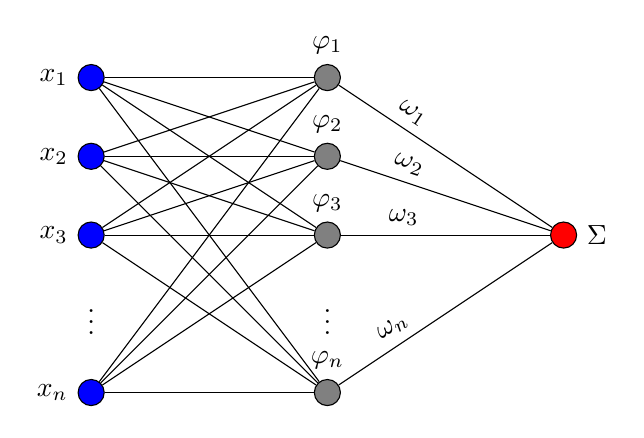
\begin{tikzpicture}
[   cnode/.style={draw=black,fill=#1,minimum width=3mm,circle},
]
\node[cnode=red,label=0:$\Sigma$] (s) at (6,-3) {};
\node at (0,-4) {$\vdots$};
\node at (3,-4) {$\vdots$};
\foreach \x in {1,...,4}
{   \pgfmathparse{\x<4 ? \x : "n"}
    \node[cnode=blue,label=180:$x_{\pgfmathresult}$] (x-\x) at (0,{-\x-div(\x,4)}) {};
    \node[cnode=gray,label=90:$\varphi_{\pgfmathresult}$] (p-\x) at (3,{-\x-div(\x,4)}) {};
    \draw (p-\x) -- node[above,sloped,pos=0.3] {$\omega_{\pgfmathresult}$} (s);
}
\foreach \x in {1,...,4}
{   \foreach \y in {1,...,4}
    {   \draw (x-\x) -- (p-\y);
    }
}
\end{tikzpicture}
\end{comment}
$\T^{(i)}$ in Equation~\ref{eq:NNconcat} stands for the parameters in layer i with $\T^{(i)}_{j,:}$
being the parameters the $j$-th neuron in that layer~\citep{goodfellow_deep_2016}.
The forwardpropagation can also be described by a computational graph~\citep{goodfellow_deep_2016}.
% FIXME: computational graph figure

The term \ac{DNN} comes from adding many hidden layers to the \ac{NN}~\citep{shrestha_review_2019}.
This allows for a more complicated function and better developed features or representations that
are extracted from the input feature vector $\x$~\citep{oyedotun_deep_2015}.
The \ac{DNN} can be trained as a whole, thus making feature engineering redundant in contrast to
normal \ac{ML} algorithms~\citep{arpteg_software_2018}.
The training algorithm is called backpropagation.
The training error is calculated through the objective function and is propagated
in conjunction with the output of forwardpropagation on each neuron~\citep{goodfellow_deep_2016}.
For this the chain rule of calculus can be used to modularly, recursively used to propagate the
loss backwards to use \ac{GD}.
The upstream gradient that is coming from neurons in the next layer is multiplied with the
jacobian matrix of the current neuron to produce the downstream gradient that is then used by
the preceding layer~\citep{boue_deep_2018,goodfellow_deep_2016}.
\begin{equation}\label{eq:backPropNeuronW}
    \frac{\delta f}{\delta\w} = \frac{\delta f}{\delta\z} \frac{\delta\z}{\delta\w}
\end{equation}
\begin{equation}\label{eq:backPropNeuronX}
    \frac{\delta f}{\delta\x} = \frac{\delta f}{\delta\z}\frac{\delta\z}{\delta\x}
\end{equation}
The result of Equation~\ref{eq:backPropNeuronW} is used to update the neuron's weights \w\ while
the result of Equation~\ref{eq:backPropNeuronX} is used for further propagation~\citep{boue_deep_2018}.
This calculation is performed until the first layer of the computational graph is
reached~\citep{goodfellow_deep_2016}.
Note that the algorithm can be performed with tensors of arbitrary
dimensionality~\citep{goodfellow_deep_2016}.

CNN
\begin{itemize}
    \item usage
    \item components: conv layer (1d \& 2d), pooling layer, normailization, ReLU, fully connected layer
    \item architectures ResNet
        \begin{itemize}
            \item aggressive downsampling
            \item $3\times3$ best kernel size
            \item Gradient saving $\rightarrow$ Res block, Res Bottleneck, Res Grouped
        \end{itemize}
\end{itemize}

RNN
\begin{itemize}
    \item usage
    \item LSTM:\ structure, rollout
    \item attention
\end{itemize}

Transformers
\begin{itemize}
    \item usage
    \item components: embedding (input \& output), positional encoding, multi-head attention,
        fully connected layer
    \item architecture: embedding \& positional encoding $\rightarrow$ encoder block
        $\rightarrow$ decoder block $\rightarrow$ softmax \& right shifting
\end{itemize}

\section{Scene Text Spotting}
%% intro
% def, ocr vs sts
\ac{OCR} is the concept of extracting typed, handwritten or printed text
from an image~\citep{zhao_improving_2020}.
Achieving satisfactory performance of \ac{OCR} systems in natural scenes is still
challenging~\citep{zhao_improving_2020, chen_text_2021}.
Such scenes entail natural scenes captured by a camera~\citep{chen_text_2021, baek_what_2019}.
The difficulties arise from diviersity and variability of text, complexity and interference from
backgrounds and imperfect imaging conditions.
In these conditions \ac{OCR} is known as \ac{STS}~\citep{long_scene_2021}.
% DL influence
Before the advent of \ac{DL}, researchers in the field had to hand-craft features~\citep{long_scene_2021}.
\ac{DL} automates the feature generation process with its representation and learning
capabilities~\citep{long_scene_2021,goodfellow_deep_2016}.
Because of this, \ac{DL} methods are the prefered tools for performing \ac{STS}~\citep{long_scene_2021}.
\ac{OCR} and \ac{STS} are often divided into two subcategories (Scene) Text Detection and (Scene)
Text Recognition~\citep{zhao_improving_2020, long_scene_2021,chen_text_2021}.
% STD, STR, end to end
For \ac{STD} the task is to localize text instances in the image, whereas the \ac{STR} task
is to recognize/categorize text from already cropped images~\citep{chen_text_2021}.
Note that a system which performs both \ac{STR} and \ac{STD} in one continuous pipeline are called
end-to-end approaches~\citep{chen_text_2021}.
% FIXME: figure with two images: multiple text instances --- cropped image with one

%% evaluation metrics
% XXX: properties and pros for different metrics
% XXX: table with task, metric, properties/why it's used
To assess the performance of the developed approaches, the right evaluation metrics
have too be used.
% STD
The popular protocols Precision, Recall and the \fone\ are used for
comparison among approaches for \ac{STD}~\citep{long_scene_2021}.
The metrics are derived with values from the confusion matrix (see
Tabel~\ref{tb:confusionMatrix})~\citep{davis_relationship_2006}.
\begin{table}[ht]
    \centering\scriptsize
    \makebox[\textwidth][c]{\begin{tabular}{cccc}
        \toprule
                  & & \multicolumn{2}{c}{\textbf{Ground Truth}} \\
                  & & positive & negative \\
        \midrule
            \textbf{Prediction} & \multicolumn{1}{c|}{\makecell{positive\\negative}}
                            & \makecell{True Positive \\ False Negative }
                            & \makecell{False Positive \\ True Negative} \\
        \bottomrule
    \end{tabular}}
    \caption{Confusion Matrix\label{tb:confusionMatrix}}
\end{table}
\begin{equation}\label{eq:P}
    \text{Precision}=\frac{\text{True Positive}}{\text{True Positive + False Positive}}
\end{equation}
\begin{equation}\label{eq:R}
    \text{Recall}=\frac{\text{True Positive}}{\text{True Positive + False Negative}}
\end{equation}
\begin{equation}\label{eq:f1}
    F_1\text{-Score}=\frac{2\cdot \text{Precision}\cdot \text{Recall}}{\text{Precision}+\text{Recall}}
\end{equation}
The difference of metrics for the task manifests itself in the way the values of the confusion matrix
are calculated~\citep{long_scene_2021}.
Note that the tradeoff between False Positives and Fales Negatives manifests itself in the
Precision-versus-Recall curve~\citep{su_relationship_2015}.
\fone\ is also refered to as the harmonic mean (between Precision and Recall)~\citep{he_icpr2018_2018}.
% FIXME: PvR curve figure
% FIXME: introduce ROC curve --- ratio of true positive rate and false positive rate, and
%           relationship to PvR curve/AP
\ac{STD} differs mostly in the way the protocols match the prediction to the ground
truth~\citep{long_scene_2021}.
Detectors have multiple predictors which regress the placing and sizing of bounding boxes.
More information on this will follow in Chapter~\ref{ch:research}.
Matching is the process of assigning a bounding box prediction to the ground
truth, like in e.g.~\cite{liu_ssd_2016,liao_textboxes_2018}.
The PASCAL approach defines the \ac{IOU} (see Equation~\ref{eq:iou}).
\begin{equation}\label{eq:iou}
    \ac{IOU}=
            \frac{\text{area of intersection between truth and prediction}}{\text{area of union
            between truth and prediction}}
\end{equation}
For PASCAL, the prediction will be matched, if the \ac{IOU} value is larger than a
threshhold~\citep{long_scene_2021}.
A match is considered a True Positive, the other values are assigned accordingly~\citep{sun_icdar_2019}.
% more BB have IOU>threshhold -> depending on situation all or greatest value
Other evaluation approaches are mostly based on \ac{IOU}, e.g. MSRA-TD 500 evaluates the rotation
from the bounding box, compared to the truth in addition to the \ac{IOU}
threshhold~\citep{long_scene_2021}.
\cite{long_scene_2021} argues that researchers in the field of \ac{STD} should consider \ac{AP}
as the main evaluation protocol rather than \fone.
According to~\cite{su_relationship_2015}, \ac{AP} can be considered the area under the
Precision-versus-Recall curve.
\fone\ on the other hand only considers singular instances on that curve~\citep{long_scene_2021} and
is sensitive to the tradeoff while \ac{AP} is invariant to it~\citep{shi_icdar2017_2017}.
% STR
For \ac{STR} the evaluation can be based on character-level or word-level.
There is no need to match ground truth to prediction, as the image is already
cropped~\citep{long_scene_2021}.
The equations~\ref{eq:wordRecognitionAccuracy} and~\ref{eq:wordErrorRate} show metrics based on
word level~\citep{chen_text_2021}.
\begin{equation}\label{eq:wordRecognitionAccuracy}
\text{Word Recognition Accuracy} = \frac{\text{correctly recognized words}}{\text{total words}}
\end{equation}
\begin{equation}\label{eq:wordErrorRate}
    \text{Word Error Rate} = 1 - \text{Word Recognition Accuracy}
\end{equation}
An example for a character-based metric would be $1 - $NED where \ac{NED}
calculates the distance between prediction and ground truth (see Equation~\ref{eq:ned}).
\begin{equation}\label{eq:ned}
    \text{NED} = \frac{1}{N}\sum_{i=1}^N \frac{D(s_i,\hat{s}_i)}{\max(l_i,\hat{l_i})}
\end{equation}
D denotes the Levenshtein distance, s denotes the text, l denotes the text length and N is the total
number of text lines~\citep{shi_icdar2017_2017}.
For \ac{STR} \ac{NED} is used over the whole dataset~\citep{karatzas_icdar_2013}.
\ac{STS} is oriented to both \ac{STD} and \ac{STR}.
The prediction has to be matched to the ground truth like for \ac{STD}~\citep{long_scene_2021}.
For comparing predictions and matched the respective ground truths that have been matched, \ac{NED} is
used~\citep{chen_text_2021}.
For end-to-end recognition~\citep{karatzas_icdar_2013,karatzas_icdar_2015}, the main evaluation
protocols that are used include Precision, Recall, \fone\ and \ac{AED}~\citep{chen_text_2021}.
A sample is considered a True positive if the \ac{NED} distance between predictions and
matched ground truths is equal to 0~\citep{sun_icdar_2019} (on sample can have multiple text instances).
\ac{AED} is the sum of \ac{NED} values devided by the number of pictures~\citep{chen_text_2021}.
Note that competitions often define their own variants of the metrics,
e.g.~\cite{he_icpr2018_2018,shi_icdar2017_2017}.
Case sensitivity and matching criteria are examples for changing properties of metrics.

To compare approaches with these metrics benchmark datasets are used which have different
characteristics.
\begin{table}[ht]
    \centering\scriptsize
    \begin{tabular}{p{.2\textwidth}p{.05\textwidth}p{.05\textwidth}p{.15\textwidth}p{.3\textwidth}}
        \textbf{Dataset (year)}&\textbf{\ac{STD}}&\textbf{\ac{STR}}&\textbf{Text Orientation}
                               &\textbf{Characteristics} \\
        \toprule
        ICDAR (2013) & \checkmark& \checkmark&Horizontal& Stroke labels \\
        ICDAR (2015) & \checkmark& \checkmark&Multi-oriented& Bad image quality\\
        ICDAR MLT (2019) & \checkmark&\checkmark&Multi-oriented& Multilingual \\
        SCUT CTW1500 (2017)& \checkmark& &Curved& --- \\
        Total-Text (2017) & \checkmark& \checkmark&Curved& Polygon labeles \\
        IIIT 5K-Word (2012) & &\checkmark&Horizontal&Cropped \\
        \bottomrule
    \end{tabular}
    \caption{Benchmark datasets and their properties\label{tb:datasets}}
\end{table}
Table~\ref{tb:datasets} lists a couple of influencial benchmark datasets along with their key
properties.
The second and third column indicate whether the dataset provides annotations for the tasks.
The Text Orientation column specifies the most complicated orientation that is present in the dataset
(Curved $\subset$ Multi-oriented $\subset$ Horizontal).

\begin{figure}[h]
    \centering\scriptsize
    \subfigure[\scriptsize ICDAR (2013)~\citep{karatzas_icdar_2013}\label{fig:ICDAR-2013}]
        {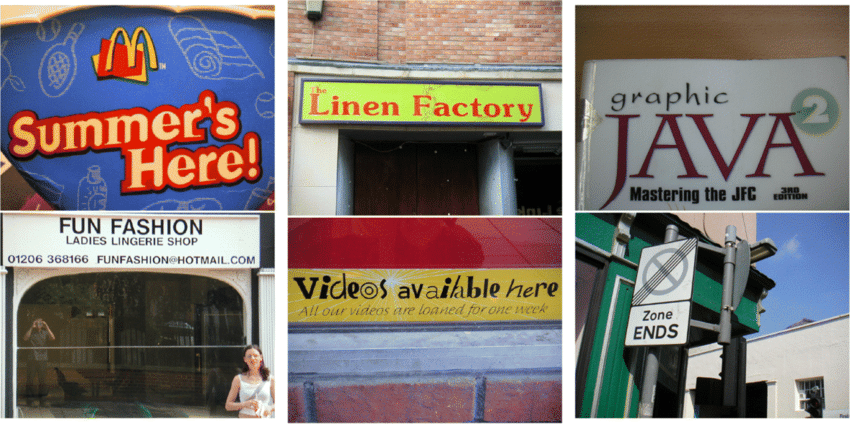
\includegraphics[width=0.40\textwidth]{img/Dataset-Examples/icdar-2013-examples.png}}
    \subfigure[\scriptsize IIIT 5k Word (2012)~\citep{mishra_scene_2012}\label{fig:IIIT-5k}]
        {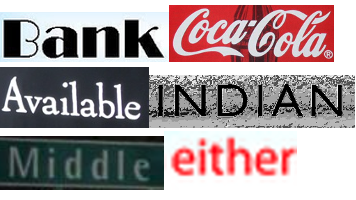
\includegraphics[width=0.40\textwidth]{img/Dataset-Examples/IIIT-5k-word-examples.png}}
    \subfigure[\scriptsize ICDAR (2015)~\citep{karatzas_icdar_2015}\label{fig:ICDAR-2015}]
        {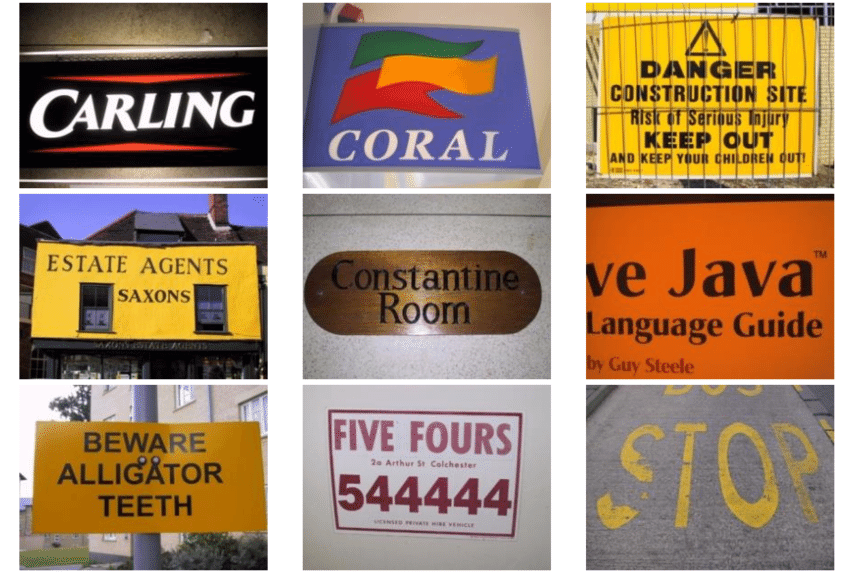
\includegraphics[width=0.40\textwidth]{img/Dataset-Examples/icdar-2015-examples.png}}
    \subfigure[\scriptsize ICDAR MLT (20159)~\citep{nayef_icdar2019_2019}\label{fig:ICDAR-2015}]
        {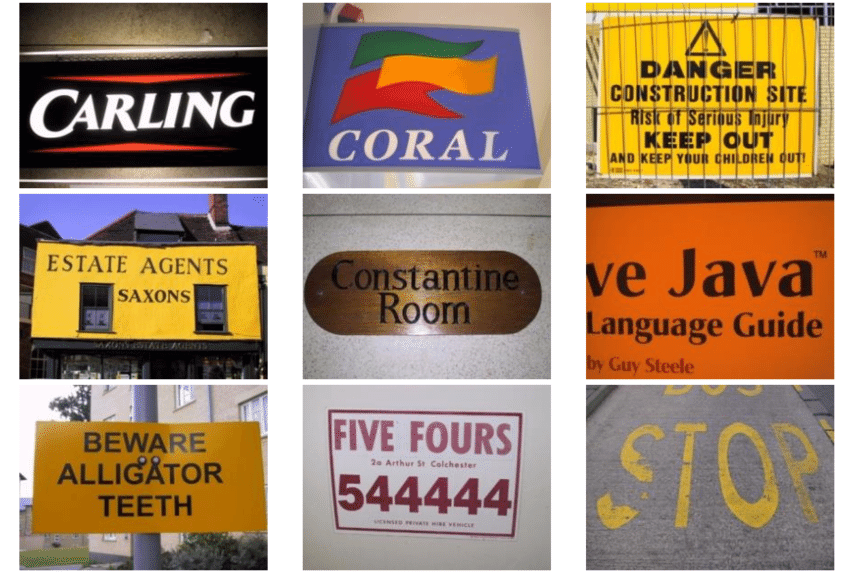
\includegraphics[width=0.40\textwidth]{img/Dataset-Examples/icdar-2015-examples.png}}
    \subfigure[\scriptsize SCUT CTW1500 (2017)~\citep{yuliang_detecting_2017}\label{fig:SCUT-CWT1500}]
        {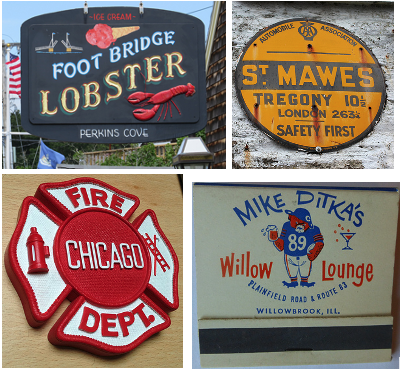
\includegraphics[width=0.40\textwidth]{img/Dataset-Examples/SCUT-CWT1500-examples.png}}
    \subfigure[\scriptsize Total Text (2017)~\citep{chan_total-text-dataset_2022}\label{fig:total-text}]
        {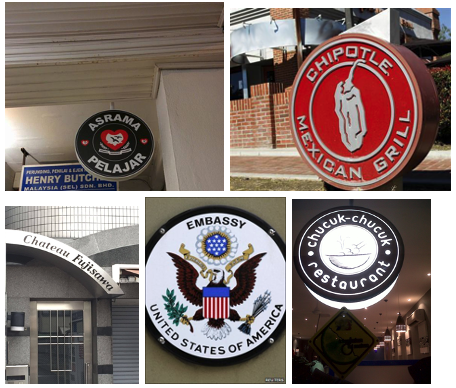
\includegraphics[width=0.40\textwidth]{img/Dataset-Examples/Total-Text-examples.png}}
    \caption{Benchmark Data Set Examples\label{fig:dataset-examples}}
\end{figure}
